\subsection{Aantal verborgen knopen}
Het aantal verborgen knopen kan voor veel variatie in de antwoorden zorgen. Hoe meer verborgen knopen zich in het netwerk bevinden, hoe meer gewichten het netwerk heeft om bij te stellen. Dit leidt tot antwoorden die meer nauwkeurig zijn.

\begin{table}[ht]
    \centering
      $\begin{array}{c||c|c |}
        \text{Aantal verborgen knopen} & \text{Aantal correct} & \text{Percentage \% correct} \\ \hline
        1 & 0 & 0 \\ \hline
        4 & 19 & 38 \\ \hline
        7 & 30 & 60 \\ \hline
        10 & 29 & 58 \\ \hline
        13 & 35 & 70 \\ \hline
        16 & 42 & 84 \\ \hline
        19 & 43 & 86 \\ \hline
        22 & 43 & 86 \\ \hline
        25 & 42 & 84 \\ \hline
      \end{array}$
    \caption{Aantal correcte antwoorden over 50 executies met verschillende aantallen verborgen knopen}
    \label{tab:hidden}
\end{table}

\begin{figure}[ht]
    \centering
    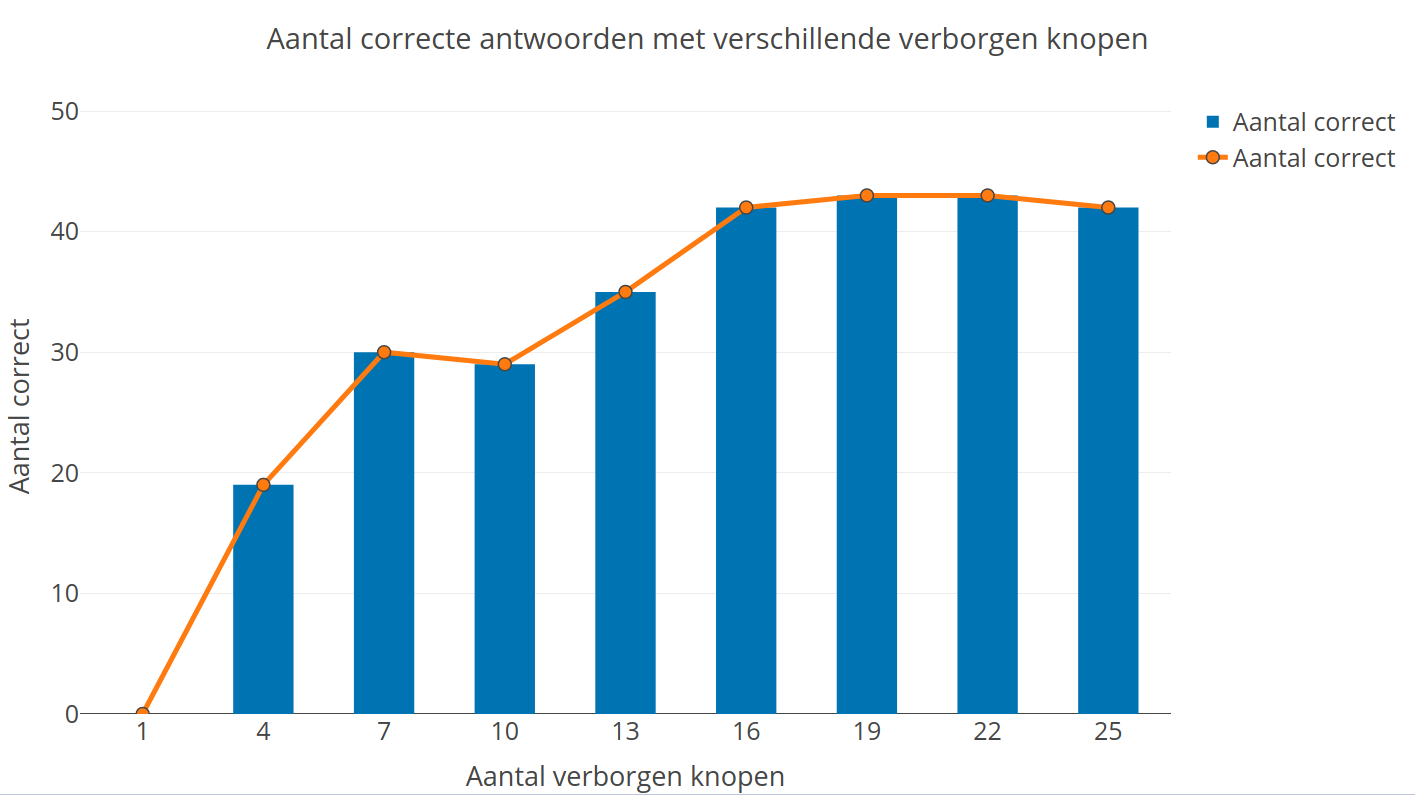
\includegraphics[scale=0.3]{graphs/knopen.png}
    \caption{Aantal correcte antwoorden over 50 executies met verschillende aantallen verborgen knopen}
    \label{fig:hidden}
\end{figure}

Zoals verwacht, hoe meer verborgen knopen er in het netwerk zijn, hoe beter het netwerk een correct antwoord kan geven. We zien in Figuur \ref{fig:hidden} dat de piek zich rondom de 19-22 knopen bevindt waarna het stabiel blijft. 
